\section{Architektury MVC i MVVM w aplikacjach .NET}

\subsection{Wprowadzenie}
Wzorce projektowe MVC (Model–View–Controller) i MVVM (Model–View–ViewModel) są podstawą nowoczesnego tworzenia aplikacji w środowisku .NET.  
MVC stosuje się głównie w aplikacjach webowych (ASP.NET Core), natomiast MVVM w aplikacjach desktopowych i mobilnych (WPF, MAUI).

\subsection{Wzorzec MVC – Model, View, Controller}
\textbf{MVC} oddziela warstwy aplikacji w celu poprawy czytelności i testowalności kodu.

\begin{itemize}
    \item \textbf{Model} – reprezentuje dane oraz logikę biznesową.
    \item \textbf{View} – odpowiada za prezentację danych użytkownikowi.
    \item \textbf{Controller} – przetwarza żądania, wywołuje odpowiednie metody modelu i przekazuje dane do widoku.
\end{itemize}

\begin{lstlisting}[language=C, caption={Przykładowy kontroler w ASP.NET Core}]
public class ProductsController : Controller
{
    private readonly IProductService _service;
    public ProductsController(IProductService service)
    {
        _service = service;
    }

    public IActionResult Index()
    {
        var products = _service.GetAll();
        return View(products);
    }

    public IActionResult Details(int id)
    {
        var product = _service.GetById(id);
        if (product == null)
            return NotFound();
        return View(product);
    }
}
\end{lstlisting}

\begin{center}
\begin{tikzpicture}[node distance=2cm, every node/.style={align=center}]
\node (client) [draw, rounded corners, fill=blue!10, text width=3cm] {Przeglądarka};
\node (controller) [draw, rounded corners, fill=green!10, below of=client, text width=3cm] {Controller};
\node (model) [draw, rounded corners, fill=orange!10, below of=controller, text width=3cm] {Model};
\node (view) [draw, rounded corners, fill=yellow!10, right of=controller, xshift=3.5cm, text width=3cm] {View (HTML)};

\draw[->, thick] (client) -- (controller);
\draw[->, thick] (controller) -- (model);
\draw[->, thick] (model) -- (controller);
\draw[->, thick] (controller) -- (view);
\draw[->, thick] (view) -- (client);
\end{tikzpicture}
\end{center}

\subsection{Wzorzec MVVM – Model, View, ViewModel}
\textbf{MVVM} jest rozwinięciem koncepcji MVC, zaprojektowanym dla aplikacji z interfejsem graficznym (UI).  
Oddziela logikę prezentacji (ViewModel) od widoku (View), dzięki czemu można testować logikę bez interakcji z interfejsem użytkownika.

\begin{itemize}
    \item \textbf{Model} – dane aplikacji i logika biznesowa,
    \item \textbf{ViewModel} – warstwa pośrednia między View a Modelem, implementuje \texttt{INotifyPropertyChanged},
    \item \textbf{View} – interfejs użytkownika, najczęściej w XAML.
\end{itemize}

\begin{lstlisting}[language=C, caption={Przykładowy ViewModel w WPF}]
public class MainViewModel : INotifyPropertyChanged
{
    private string _message = "Witaj w aplikacji MVVM!";
    public string Message
    {
        get => _message;
        set
        {
            _message = value;
            OnPropertyChanged(nameof(Message));
        }
    }

    public ICommand ChangeMessageCommand { get; }

    public MainViewModel()
    {
        ChangeMessageCommand = new RelayCommand(ChangeMessage);
    }

    private void ChangeMessage()
    {
        Message = "Tekst został zmieniony!";
    }

    public event PropertyChangedEventHandler? PropertyChanged;
    private void OnPropertyChanged(string propertyName)
        => PropertyChanged?.Invoke(this, new PropertyChangedEventArgs(propertyName));
}
\end{lstlisting}

\begin{lstlisting}[language=XML, caption={Fragment widoku XAML (MainWindow.xaml)}]
<Window x:Class="MVVMApp.MainWindow"
        xmlns="http://schemas.microsoft.com/winfx/2006/xaml/presentation"
        xmlns:x="http://schemas.microsoft.com/winfx/2006/xaml"
        Title="MVVM App" Height="200" Width="400">
    <Grid>
        <StackPanel HorizontalAlignment="Center" VerticalAlignment="Center">
            <TextBlock Text="{Binding Message}" FontSize="16" Margin="0,0,0,10"/>
            <Button Content="Zmień tekst" Command="{Binding ChangeMessageCommand}" Width="150"/>
        </StackPanel>
    </Grid>
</Window>
\end{lstlisting}

\subsection{Diagram przepływu MVVM}
\begin{center}
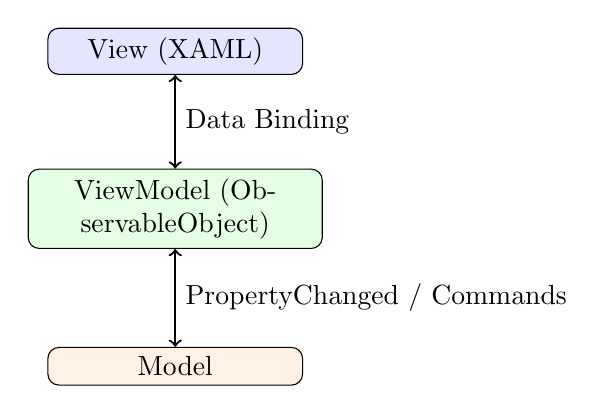
\begin{tikzpicture}[node distance=2cm, every node/.style={align=center}]
\node (view) [draw, rounded corners, fill=blue!10, text width=3cm] {View (XAML)};
\node (vm) [draw, rounded corners, fill=green!10, below of=view, text width=3.5cm] {ViewModel (ObservableObject)};
\node (model) [draw, rounded corners, fill=orange!10, below of=vm, text width=3cm] {Model};

\draw[<->, thick] (view) -- node[right]{Data Binding} (vm);
\draw[<->, thick] (vm) -- node[right]{PropertyChanged / Commands} (model);
\end{tikzpicture}
\end{center}

\subsection{Porównanie MVC i MVVM}
\begin{center}
\begin{tabular}{|p{3cm}|p{5cm}|p{5cm}|}
\hline
\textbf{Cecha} & \textbf{MVC} & \textbf{MVVM} \\
\hline
Zastosowanie & Aplikacje webowe & Aplikacje desktopowe/mobilne (WPF, MAUI) \\
\hline
Warstwa prezentacji & View + Controller & View + ViewModel \\
\hline
Powiązanie danych & Ręczne przekazywanie danych & Data Binding (TwoWay) \\
\hline
Obsługa zdarzeń & Metody kontrolera & Komendy (ICommand) \\
\hline
Testowalność logiki & Średnia & Bardzo wysoka \\
\hline
\end{tabular}
\end{center}

\subsection{Binding i konwertery danych}
Binding w MVVM umożliwia dwukierunkową synchronizację danych pomiędzy widokiem a modelem.

\begin{lstlisting}[language=C, caption={Przykład konwertera wartości}]
public class BoolInverseConverter : IValueConverter
{
    public object Convert(object value, Type targetType, object parameter, CultureInfo culture)
        => !(bool)value;

    public object ConvertBack(object value, Type targetType, object parameter, CultureInfo culture)
        => !(bool)value;
}
\end{lstlisting}

\begin{lstlisting}[language=XML, caption={Zastosowanie konwertera w XAML}]
<Button Content="Wyślij" 
        IsEnabled="{Binding IsBusy, Converter={StaticResource BoolInverseConverter}}"/>
\end{lstlisting}

\subsection{Walidacja danych}
\begin{lstlisting}[language=C, caption={Walidacja danych z użyciem DataAnnotations}]
public class User
{
    [Required]
    public string Name { get; set; } = string.Empty;

    [Range(18, 99)]
    public int Age { get; set; }
}
\end{lstlisting}

\subsection{Zalety MVVM}
\begin{itemize}
    \item Łatwe testowanie logiki prezentacji bez UI.
    \item Spójna architektura z separacją odpowiedzialności.
    \item Łatwe utrzymanie i rozwój aplikacji.
    \item Możliwość współdzielenia logiki między platformami (MAUI).
\end{itemize}

\subsection{Wady MVVM}
\begin{itemize}
    \item Większa złożoność początkowa.
    \item Trudniejsze debugowanie powiązań (bindings).
    \item Więcej kodu pomocniczego (np. RelayCommand, BaseViewModel).
\end{itemize}

\subsection{Podsumowanie rozdziału}
\begin{itemize}
    \item MVC stosujemy w aplikacjach webowych, MVVM w desktopowych i mobilnych.
    \item MVVM wprowadza binding, ICommand i testowalność logiki prezentacji.
    \item Wzorce zapewniają lepszą separację odpowiedzialności i czystszy kod.
\end{itemize}

\subsection{Pytania kontrolne}
\begin{enumerate}
    \item Jakie są trzy główne komponenty MVC i ich funkcje?
    \item W jaki sposób MVVM ułatwia testowanie aplikacji?
    \item Do czego służy interfejs \texttt{INotifyPropertyChanged}?
    \item Jak działają konwertery wartości (ValueConverter) w XAML?
    \item Jakie są różnice w przepływie danych między MVC a MVVM?
\end{enumerate}
